%%%%%%%%%%%%%%%%%%%%%%%%%%%%%%%%%%%%%%%%%%%%%%%%%%%%%%%%%%%%%%%%%%%%%%%%%%%%%%%%
% \documentclass[12pt,papel,twoside]{ibtesis}
\documentclass[12pt,screen,twoside,pagebackref]{ibtesis}
% \documentclass[12pt,papel,singlespace,oneside]{ibtesis}
% \documentclass[12pt,papel,preprint,singlespace,oneside]{ibtesis}

%\DeclareUnicodeCharacter{200B}{I~AM~HERE!!!!}
%\DeclareUnicodeCharacter{2212}{I~AM~HERE!!!!}

%%%%%%%%%%%%%%%%%%%%% Paquetes extra %%%%%%%%%%%%%%%%%%%%%%%%%%%%%%%%%%%%%%%%%%%
% Por conveniencia: aqu\'{\i} puede cargar todos los paquetes y definir los comandos 
% que necesite
\usepackage{ibextra}

%%%%%%%%%%%%%%%%%%%%%%%%%%%%%%%%%%%%%%%%%%%%%%%%%%%%%%%%%%%%%%%%%%%%%%%%%%%%%%%%
%%%%%%%%%%%%%%%%%%%%% Informacion sobre la tesis %%%%%%%%%%%%%%%%%%%%%%%%%%%%%%%
\title{Comportamientos emergentes en poblaciones de robots interactuantes}
\author{Mg. Carlos Eduardo Valencia Urbina}
\director{Dr. Pablo Martin Gleiser}
\carrera{Tesis Carrera de Doctorado en F\'{\i}sica}
\grado{Doctorando}
\laboratorio{Departamento de Física Medica -- Centro At\'{o}mico Bariloche}
\jurado{Dr.~J.~J.~Jurado (Instituto Balseiro) \\ 
Dr.~Segundo Jurado (Universidad Nacional de Cuyo)\\ 
Dr.~J.~Otro Jurado (Univ. Nac. de LaCalle)\\
Dr.~J.~L\'{o}pez Jurado (Univ. Nac. de Mar del Plata)\\
Dr.~U.~Amigo (Instituto Balseiro, Centro At\'{o}mico Bariloche)}
\palabrasclave{formato de Tesis, Lineamientos de escritura, Instituto Balseiro}
\keywords{Thesis format, Templates, Instituto Balseiro}
% Si queremos poner la fecha manualmente:
% \date{Diciembre de 2099}

%%%%%%%%%%%%%%%%%%%%%%%%%%%%%%%%%%%%%%%%%%%%%%%%%%%%%%%%%%%%%%%%%%%%%%%%%%%%%%%%
%\titlepagefalse % Si no quiere compilar la portada descomente esta linea
%\includeonly{apendices} % Compilar s\'{o}lo estos archivos 
\graphicspath{{figs/}} % Lugar donde encontrar las figuras generales (se puede poner uno en cada cap{\'{\i}}tulo)
%%%%%%%%%%%%%%%%%%%%%%%%%%%%%%%%%%%%%%%%%%%%%%%%%%%%%%%%%%%%%%%%%%%%%%%%%%%%%%%%


\begin{document}

% Dentro del environment 'preliminary' va:
% la dedicatoria, resumen, abstract, indices

\begin{preliminary}

% Escriba su dedicatoria
\dedicatoria{
A mi familia\\
A mis amigos\\
A todos los que me conocen\\
A toda esa otra gente que no
}

%%% \'{I}ndices %%%%

%\begin{abreviaturas}
                                %Abreviaturas
%\end{abreviaturas}

\tableofcontents                %\'{I}ndice

\listoffigures                  %Figuras

\listoftables                   %Tablas

\printglossary[type=\acronymtype]

\printglossary


\begin{resumen}%
Este es el resumen en castellano.\\
La tesis debe reflejar el trabajo desarrollado, mostrando la metodolog\'{\i}a utilizada, los resultados obtenidos y las conclusiones que pueden inferirse de dichos resultados.
\end{resumen}

\begin{abstract}%
This is the title in English:\\
The thesis must reflect the work of the student, including the chosen methodology, the results and the conclusions that those results allow us to draw.
\end{abstract}


%%% Local Variables: 
%%% mode: latex
%%% TeX-master: "template"
%%% End: 


\end{preliminary}


% Podemos usar cualquiera de los dos comandos: \input o \include para incluir el texto

\chapter{Introducción}


% aplication of percolation theory
Es un hecho de la vida, que es tan desafiante para la mente del científico como frustrante para sus aspiraciones, que la naturaleza está desordenada. Sólo en el supermercado de los teóricos podemos comprar sistemas limpios, puros, perfectamente caracterizados y geométricamente inmaculados. Un ingeniero trabaja en un mundo de compuestos y mezclas (cuánto más el biólogo). Incluso el experimentador que se enfoca en la más pura de las sustancias, ejemplificada por cristales cuidadosamente cultivados, rara vez puede escapar de los efectos de los defectos, trazas de impurezas y límites finitos. Hay pocos conceptos en la ciencia más elegantes de contemplar que una red cristalina infinita, perfectamente periódica, y pocos sistemas tan alejados de la realidad experimental. Por lo tanto, estamos obligados a aceptar estructuras desordenadas; la variación en forma y constitución a menudo está tan mal caracterizada que debemos considerarla aleatoria si queremos describirla: aparente aleatoriedad en la morfología del sistema. La morfología de un sistema tiene dos aspectos principales: la topología, la interconexión de los elementos microscópicos individuales del sistema, y la geometría, la forma y el tamaño de estos elementos individuales. Pero quizás la razón más importante del rápido desarrollo de la física estadística de los sistemas desordenados es que se ha apreciado el papel de la interconectividad de los elementos microscópicos de un sistema desordenado y su efecto sobre las propiedades macroscópicas del sistema. Esto ha sido posible a través del desarrollo y aplicación de la teoría de la percolación, el tema de este libro.





Comprender la relación entre la arquitectura y la función del cerebro es una cuestión central en la neurociencia. En esa dirección, se han dedicado importantes esfuerzos en los últimos años para mapear la estructura a gran escala de distintos organismos, incluidos los intentos de construir matrices de conectividad estructural del sistema nervioso a partir de datos de imágenes.  Sin embargo,   \textquote{al igual que los genes, las conexiones estructurales por sí solas son impotentes}; por lo tanto, \textquote{el conectoma debe expresarse en actividad neuronal dinámica para ser efectivo en el comportamiento y la cognición} \cite{sporns_discovering_2012}.


\url{https://sebastianrisi.com/self_assembling_ai/}

no de los aspectos más fascinantes de la naturaleza es que grupos con millones o incluso billones de elementos pueden autoensamblarse en formas complejas basadas solo en interacciones locales y mostrar lo que se llama un tipo colectivo de inteligencia. Por ejemplo, las hormigas pueden unirse para crear puentes o balsas para navegar por terrenos difíciles, las termitas pueden construir nidos de varios metros de altura sin un plan impuesto desde el exterior, y miles de abejas trabajan juntas como un todo integrado para tomar decisiones precisas sobre cuándo buscar alimento o un nuevo nido. Sorprendentemente, lograr estas increíbles habilidades es el resultado de seguir reglas de comportamiento relativamente simples y a través de un proceso de autoorganización, que Camazine et al. (2001) definen como:

“ Como un proceso en el que el patrón a nivel global de un sistema surge únicamente de numerosas interacciones entre los componentes de nivel inferior del sistema. Además, las reglas que especifican las interacciones entre los componentes del sistema se ejecutan utilizando solo información local, sin referencia al patrón global. En resumen, el patrón es una propiedad emergente del sistema en lugar de ser impuesto al sistema por una influencia de orden externa. “

Comprender el cerebro es uno de los problemas más desafiantes por los que un físico puede sentirse atraído. Como sistema con una cantidad astronómica de elementos, cada uno de los cuales se sabe que tiene muchas no linealidades, el cerebro exhibe dinámicas colectivas que en muchos aspectos se asemejan a algunos de los problemas clásicos bien estudiados en física estadística. La contradicción, y el punto provocador de estas notas, es que solo una minoría de las publicaciones en el campo hoy se preocupan por la comprensión de la dinámica del cerebro como un proceso colectivo. Los enfoques formales para estudiar fenómenos colectivos son uno de los temas clásicos en el centro de la física estadística, con aplicaciones recientes nuevas y exitosas en diversas áreas como la genética, la ecología, la informática, los entornos sociales y económicos. Si bien en todos estos campos existe una clara transferencia de métodos e ideas desde la física estadística, un flujo similar recién ha comenzado a impactar en la neurociencia.

¿cómo se coordinan entre sí esas miríadas de elementos e interacciones en criaturas vivas complejas?" o “¿cómo emerge un comportamiento coherente de tal sopa de componentes altamente heterogéneos? Una estrategia complementaria consiste en mirar problemas biológicos complejos desde una perspectiva global, cambiando el enfoque de detalles específicos de la maquinaria molecular a aspectos integrales.  Los enfoques sistémicos de la biología se basan en la evidencia de que algunos de los fenómenos más fascinantes de los sistemas vivos, como la memoria y la capacidad para resolver problemas, son fenómenos colectivos, derivados de las interacciones de muchas unidades básicas y podrían no reducirse a la comprensión de componentes elementales de forma individual (Bialek, 2018 ).  durante mucho tiempo han sido seducidos por la idea de adaptar conceptos y métodos de la mecánica estadística para arrojar luz sobre la organización a gran escala de los sistemas biológicos

Recordemos qué son los fenómenos emergentes. La emergencia se refiere a los patrones espaciotemporales colectivos inesperados exhibidos por grandes sistemas complejos. En este contexto, 'inesperado' muestra nuestra incapacidad (matemática y de otro tipo) para derivar tales patrones emergentes de las ecuaciones que describen la dinámica de las partes individuales del sistema. Como se discutió extensamente en otra parte 1 , 15Los sistemas complejos suelen ser grandes conglomerados de elementos que interactúan, cada uno de los cuales exhibe algún tipo de dinámica no lineal.


l punto importante es que incluir la complejidad en el modelo solo dará como resultado una simulación del sistema real, sin que ello implique ninguna comprensión de la complejidad. Los esfuerzos más significativos han sido los dirigidos a descubrir las condiciones en las que algo complejo emerge de la interacción de los elementos no complejos que lo constituyen


En muchos sistemas físicos, como los sistemas magnéticos o gravitacionales, ciertas características macroscópicas surgen de las interacciones de los elementos constituyentes de una manera que es impredecible incluso a partir de una comprensión perfecta del comportamiento de cada componente; esto se conoce como emergencia ( Chialvo, 2010). En el contexto del cerebro, los fenómenos emergentes abarcan el comportamiento y la cognición, que surgen de la interacción de la gran cantidad de neuronas en el cerebro. Abordar el estudio de los sistemas neuronales desde esta perspectiva implica estudiar el comportamiento neuronal a nivel de red o población: observar y comprender los comportamientos emergentes en el sistema en lugar de concentrarse en el comportamiento y las conexiones de cada neurona individual por sí sola. Si bien exhiben cierto poder computacional por sí mismas, las neuronas son realmente notables en su capacidad computacional cuando se toman en conjunto.
https://www.frontiersin.org/articles/10.3389/fncom.2021.611183/full







\part{Dinámica crítica del C. elegans}
\chapter{Dinámica neuronal critica}\label{titulo-cap-critico}
\graphicspath{{figs/capitulo_critico/}}

\chapterquote{Can a machine be made to be supercritical? }{Alan Turing , 1950}






\section{Introducción}

La física de sistemas complejos ha demostrado que los comportamientos colectivos pueden surgir de la interacción entre los constituyentes elementales de la materia, dando lugar a fases con diferentes niveles de orden interno. Los sistemas biológicos no son la excepción, y algunos de ellos han sido identificados como operando en la vecindad del punto crítico de una transición de fase. En este sentido, la hipótesis de la criticidad neuronal sugiere que el cerebro puede estar en un estado crítico en el límite entre diferentes tipos de dinámicas, lo que le proporcionaría un equilibrio óptimo entre robustez y flexibilidad.

En este capítulo se revisarán las bases teóricas de la física de sistemas complejos y su aplicación en biología, así como los fundamentos de la hipótesis de la criticidad neuronal y las evidencias experimentales que la respaldan.






\section{Física de sistemas complejos y transiciones de fase}

\subsection{Transiciones de fase en física}

La materia, compuesta por átomos, moléculas y electrones, puede generar diversas fases cuyo comportamiento difiere significativamente de sus componentes individuales o pequeños grupos de ellos. A nivel microscópico, los sistemas que contienen muchos componentes pueden exhibir diferentes tipos de comportamientos colectivos a nivel macroscópico, es decir, fases, con diferentes niveles de orden interno. Es importante destacar que incluso pequeños cambios en las condiciones externas, como la temperatura o la presión, pueden inducir reordenamientos estructurales drásticos, lo que se conoce como transiciones de fase.\\

En la distinción de las distintas fases de un sistema, se consideran ciertas propiedades macroscópicas medibles, conocidas como parámetros de orden. La variación de una propiedad ambiental, denominada parámetro de control, permite observar cómo dichos parámetros de orden cambian. En general, una modificación gradual en el parámetro de control se traduce en una alteración suave en los parámetros de orden. Sin embargo, existen determinados puntos donde los valores de los parámetros de orden experimentan saltos o giros abruptos (ver \Cref{fig:trancisiones}). Estos puntos marcan los límites entre diferentes fases, y desplazar el parámetro de control a través de dicho límite induce una transición de fase.\\

En función de cómo se modifiquen los parámetros de orden durante una transición de fase, esta puede ser de dos tipos. Si la transición se caracteriza por un salto en los parámetros de orden del sistema, lo que matemáticamente corresponde a una discontinuidad en el diagrama de fase, se trata de una transición de fase discontinua (ver \Cref{fig:transicionI} ). Este tipo de transiciones son denominadas a veces como transiciones de primer orden. Por otra parte, si el diagrama de fase es continuo y la transición se caracteriza por una esquina aguda (es decir, un punto de no diferenciabilidad), se trata de una transición de fase continua (segundo orden, ver \Cref{fig:transicionII}). La terminología de \textquote{primer orden} y \textquote{segundo orden} se origina en la descripción de las transiciones de fase termodinámicas, haciendo referencia a la derivada más baja de la energía libre, la cual muestra una discontinuidad en el punto crítico.\\


\begin{figure}[ht]
	\centering
	\begin{subfigure}[b]{0.45\textwidth}
		\centering
		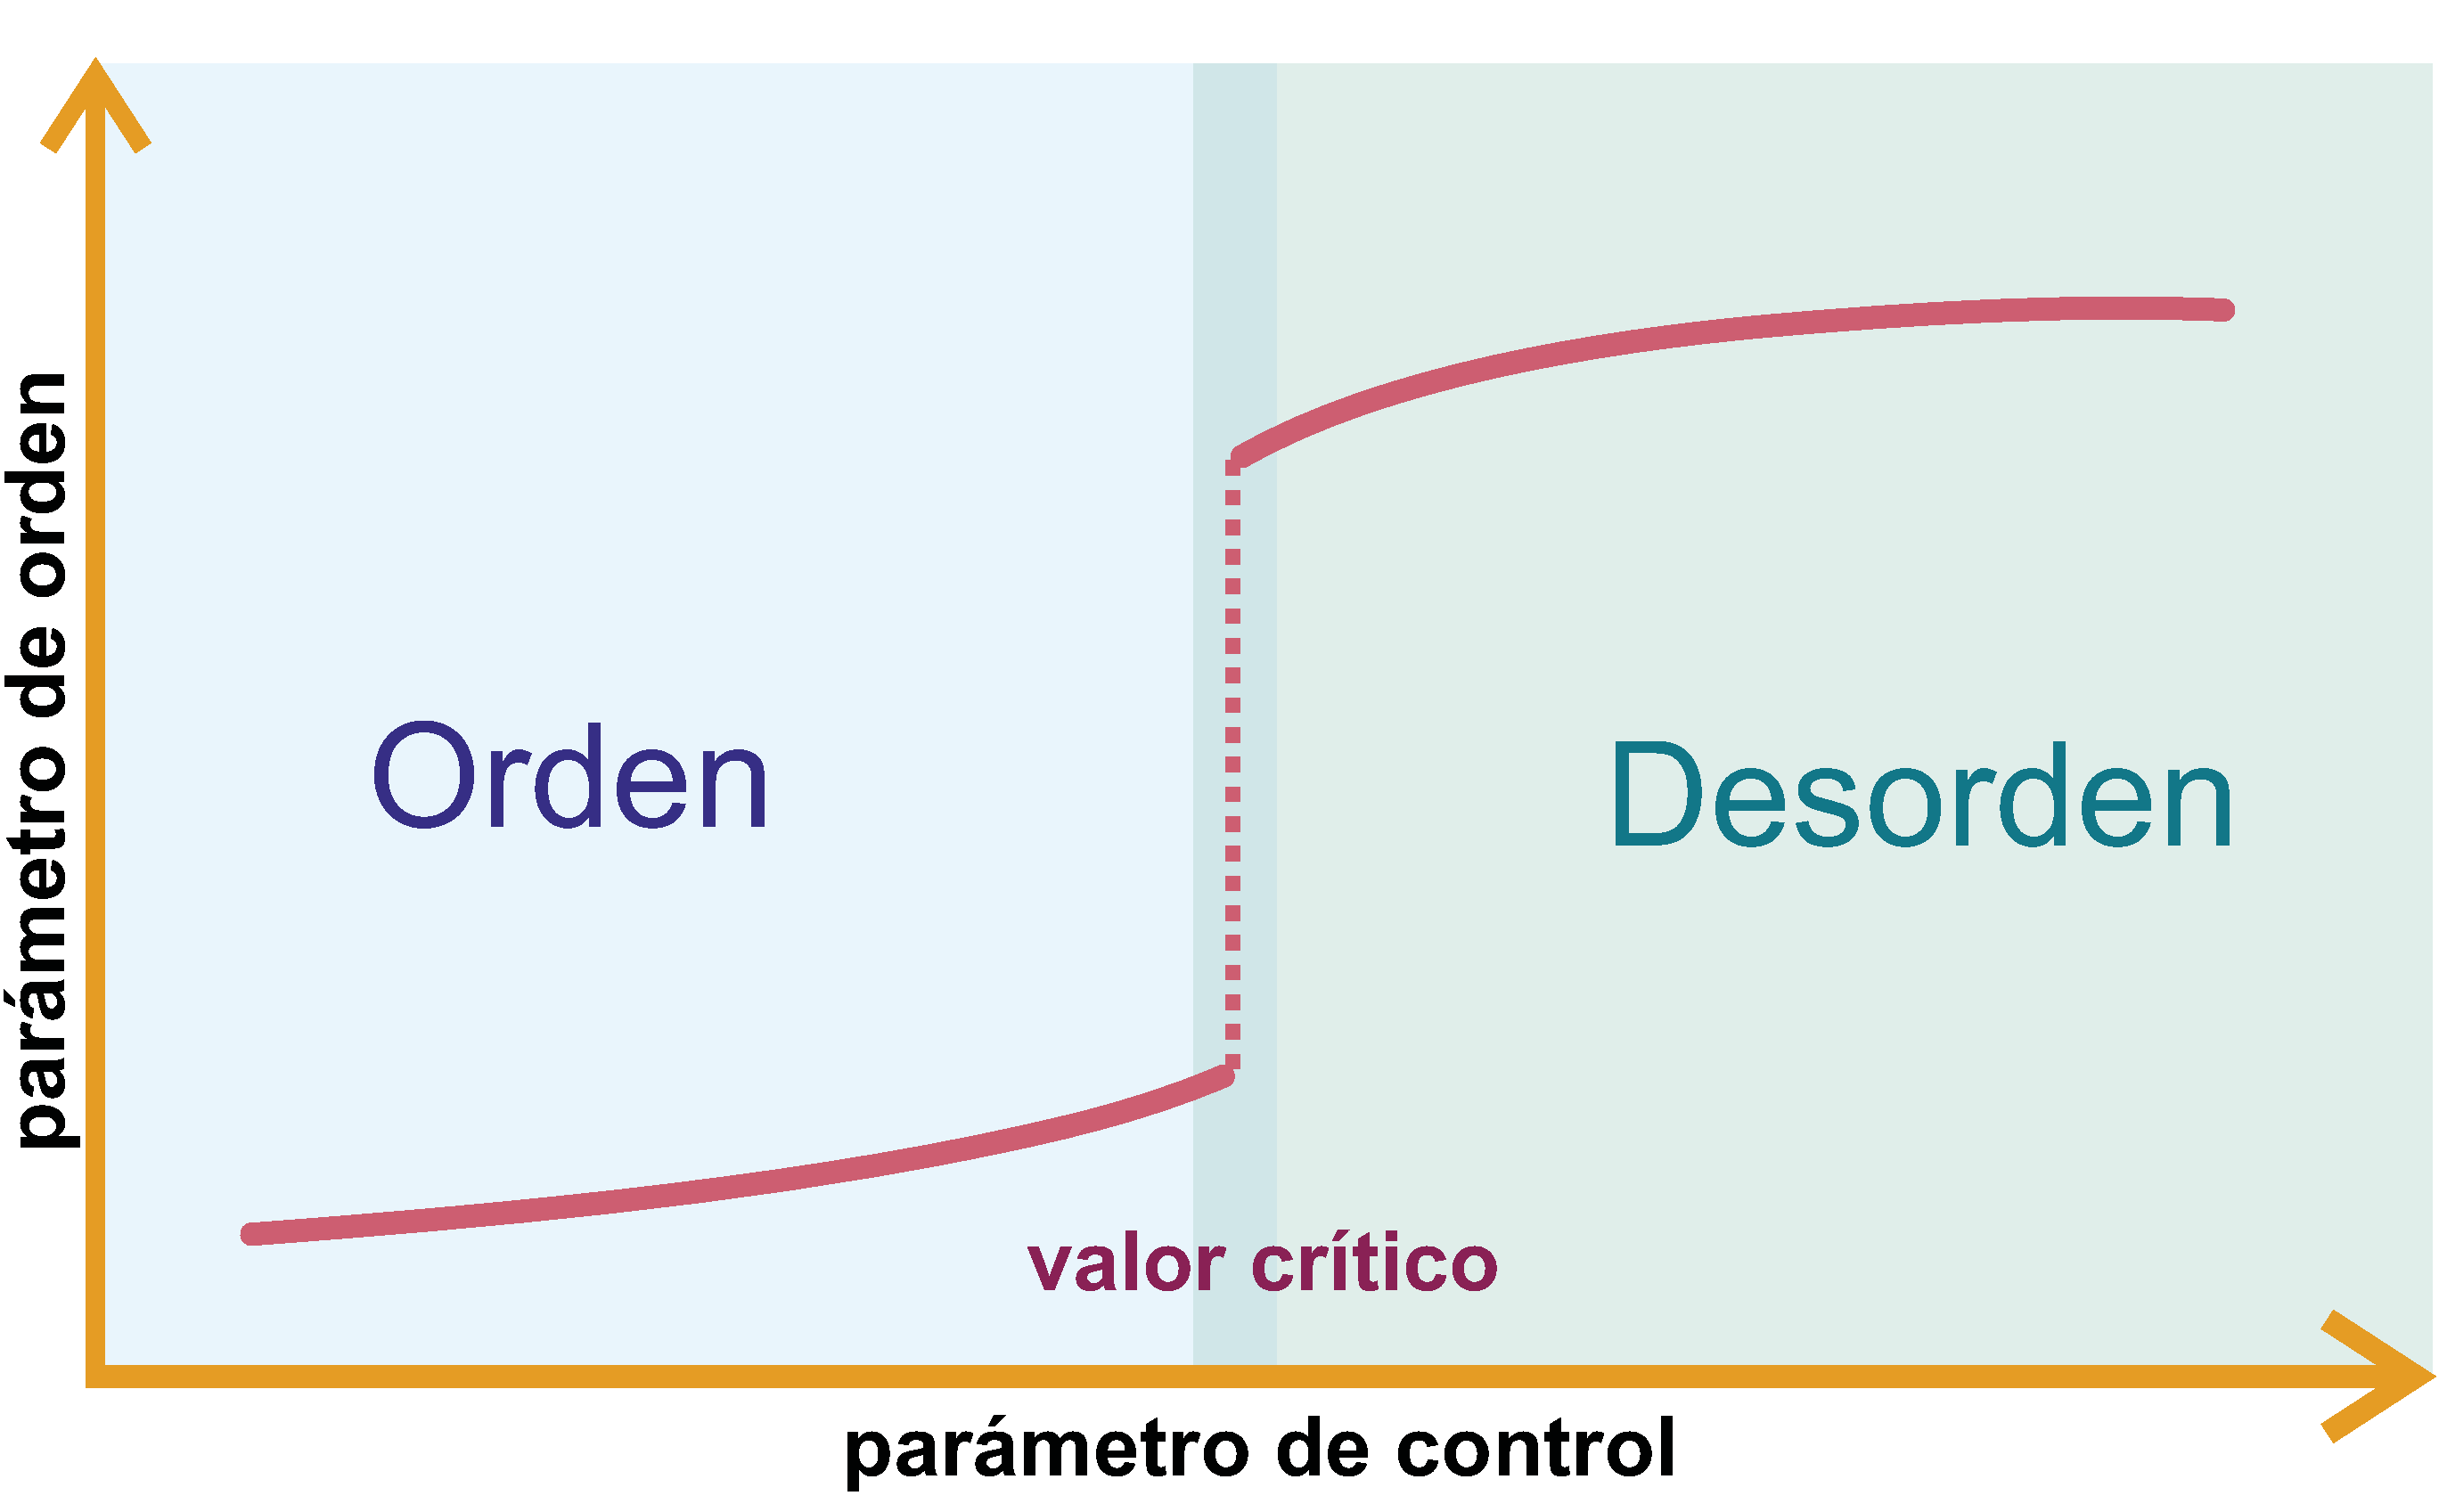
\includegraphics[width=\textwidth]{transiciones_fases_tipo_I.pdf}
		%\caption{transiciones de fase de primer orden}
		\caption{}
		\label{fig:transicionI}
	\end{subfigure}
	\begin{subfigure}[b]{0.45\textwidth}
		\centering
		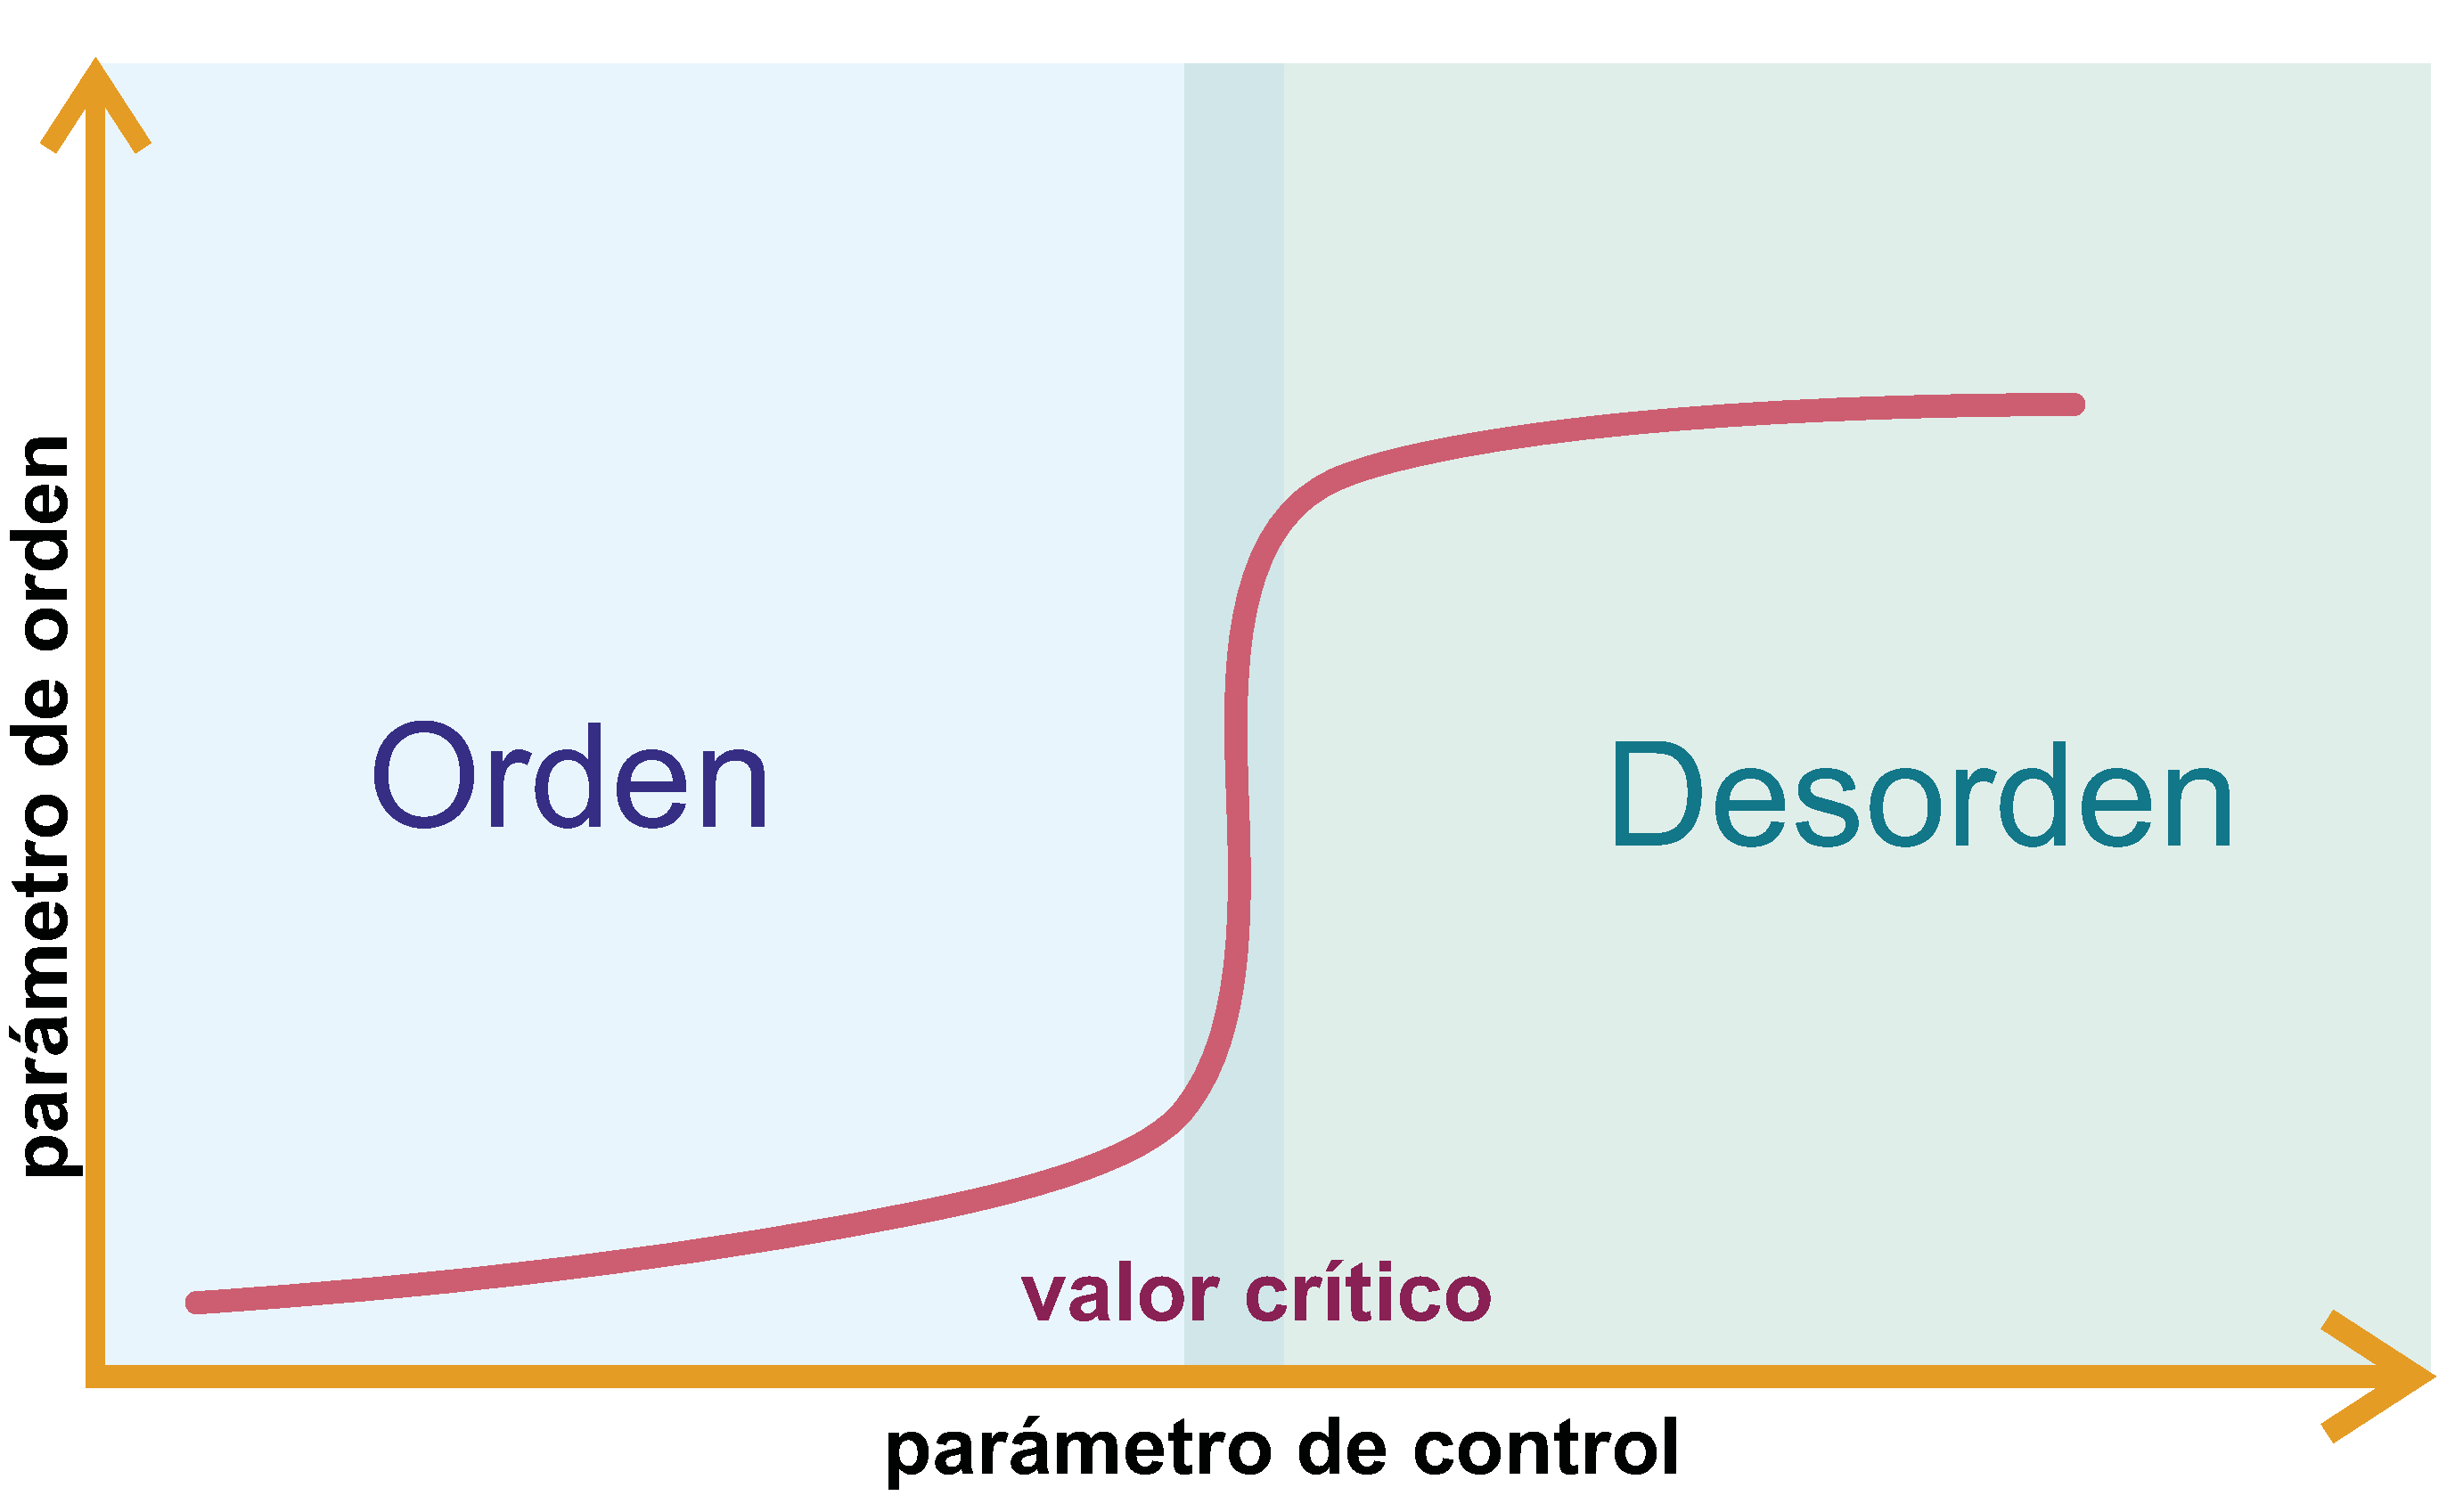
\includegraphics[width=\textwidth]{transiciones_fases_tipo_II.pdf}
		%\caption{transiciones de fase de segundo orden}
		\caption{}
		\label{fig:transicionII}
	\end{subfigure}
	\caption[Representaciones esquemáticas de transiciones de fase de primer y segundo orden.]{Representaciones esquemáticas de transiciones de fase de primer y segundo orden. La figura muestra dos ejemplos de transiciones de fase que ocurren en sistemas termodinámicos. En (a), se ilustra una transición de fase de primer orden, donde el parámetro de orden experimenta un cambio abrupto en su valor crítico del parámetro de control. En contraste, en (b) se muestra una transición de fase de segundo orden, donde el parámetro de orden varía suavemente a medida que cambia el parámetro de control.}
	\label{fig:trancisiones}
\end{figure}

Si un sistema exhibe una transición de fase continua, entonces puede existir en un punto crítico que se encuentra exactamente en la frontera entre dos fases distintas. Este estado límite, conocido como estado crítico, se caracteriza por la presencia de fluctuaciones importantes en el valor del parámetro de orden en el rango crítico, lo cual refleja la pérdida de simetría del sistema que ocurre durante las transiciones de fase. Por consiguiente, se considera que los estados críticos se encuentran en la frontera del caos. Las transiciones de fase críticas son especialmente interesantes debido al comportamiento crítico que se manifiesta en las grandes fluctuaciones del parámetro de orden, las cuales exhiben escalamiento de ley de potencia (Figura 1C).\\



\subsection{Transiciones de fase en biología}


El principio de universalidad es un concepto ampliamente aceptado en la física que establece que las características relevantes de los fenómenos a gran escala son altamente insensibles a los detalles específicos del modelo y se comparten entre sistemas aparentemente distintos. Siguiendo este principio, se ha propuesto una hipótesis controvertida, pero ampliamente investigada, según la cual algunos sistemas biológicos pueden obtener beneficios funcionales significativos al operar cerca del punto crítico de una transición de fase \cite{munoz_colloquium_2018,hidalgo_information-based_2014,kauffman_origins_1993,bak_how_1996,chialvo_brain_2008,chialvo_emergent_2010,plenz_critical_2013,niebur_criticality_2014,shew_functional_2013,cocchi_criticality_2017,zimmern_why_2020}. En particular, estos sistemas operarían en el límite entre una fase activa o caótica, en la que las fluctuaciones son amplificadas y la información se corrompe, y una fase inactiva u ordenada, en la que las fluctuaciones se amortiguan rápidamente y se reduce la capacidad de respuesta y adaptación. Se han identificado varios ejemplos de tales transiciones, como se resume en el \cref{table:transiciones_biologicas}.\\



% primer estilo 
%row{odd} = {bg=azure8},
%row{1} = {bg=azure3, fg=white, font=\sffamily},

% segundo estilo 

%row{odd} = {bg=red8},
%row{even} = {bg=red9},
%row{1} = {bg=red3, fg=white, font=\sffamily}

% tercer estilo 

%row{odd} = {bg=gray8},
%row{even} = {bg=gray9},
%row{1} = {bg=red3, fg=white, font=\sffamily},

%otra 

%row{odd} = {bg=teal9},
%row{1} = {bg=teal3, fg=white, font=\sffamily},
\begin{table}[h!]
	\centering
		\caption[Ejemplos seleccionados de transiciones de fase en biología.]{ Ejemplos seleccionados de transiciones de fase en biología, adaptado de Heffern et al\protect{\cite{heffern_phase_2021}}.}
\begin{tblr}{colspec={X[2,l]X[2,l]X[2,l]X[l]},
row{odd} = {bg=gray8},
row{even} = {bg=gray9},
row{1} = {bg=red3, fg=white, font=\sffamily},
}
	sistema	& parámetro de control	  &   parámetro de orden	& referencias seleccionadas
	  \\
	
	Fusión de la membrana plasmática	 & Temperatura	  &  Fluidez &    \cite{de_kruyff_effect_1972} \\
	

	Sincronización neuronal	 &   Fuerza sináptica; relación de excitación a inhibición	 &  Sincronización de tasas de disparo	 &    \cite{adhikari_time-delay-induced_2011,baumgarten_critical_2019}\\
	
	{Agrupamiento\\/enjambre}	 & Densidad; ruido en la percepción del comportamiento de los vecinos	  & Alineación de patrones de vuelo	  &   \cite{cavagna_scale-free_2010,bahar_flocking_2018,attanasi_finite-size_2014}  \\
	
	Rigidez de actina	 &   Densidad	 &   Rigidez &   \cite{gurmessa_triggered_2019,hussain_spatiotemporal_2013}  \\
	
Colapso de la población microbiana	 	&  Nivel de estrés	 & Crecimiento  &  \cite{mensonides_metabolic_2002,ordway_phase_2020}  \\
	
	Evolución cultural	 &  Cambios en el \gls{fitness} acompañado de \gls{epistasis} entre rasgos culturales	 &  Paradigma cultural	 & \cite{pascual_epistasis_2020}    \\
	
	
Rasgos del fitoplancton	 	& Condiciones de luz	  &   Contenido de clorofila	&  \cite{held_second-order_2020}  \\
	
	Colapso de la población de megafauna	 &   Variado& Tamaño de la poblacion	  &  \cite{hein_population_2019,lauerburg_socio-ecological_2020,heinze_quiet_2021}   \\
	
	Percolación de rigidez en embriogénesis de pez cebra	 &  Conectividad celular dependiente de la adhesión	 & Viscosidad del tejido, tamaño del grupo	  &  \cite{petridou_rigidity_2021}   \\
	
	\end{tblr}
	\label{table:transiciones_biologicas}
\end{table}

Existen varios experimentos que respaldan esta hipótesis. Algunos de estos ejemplos incluyen las transiciones de fase de sincronización en osciladores biológicos colectivos, como los relojes circadianos \cite{garcia-ojalvo_modeling_2004}; las transiciones de percolación de fibras en tejidos conectivos, como el colágeno \cite{forgacs_phase_1991,newman_phase_2004,alvarado_molecular_2013}; la transición de fase de fusión en hebras de ADN \cite{magee_jr_theory_1963,li_phase_2006}; las transiciones entre diferentes regímenes dinámicos, como las oscilaciones y los estallidos, en redes neuronales \cite{kelso_phase_1984,freeman_metastability_2005,rabinovich_dynamical_2006,werner_metastability_2007,adamatzky_chaos_2013,haken_principles_1996}; los patrones de expresión génica \cite{tsuchiya_self-organizing_2016};  el agrupamiento bacteriano \cite{larkin_signal_2018,ordway_phase_2020}  y la formación de colonias de C. elegans \cite{chen_c_2021}. Para obtener una revisión más completa de las aplicaciones de las transiciones de fase a problemas biológicos, se recomienda consultar la obra de Heffern et al \cite{heffern_phase_2021}.\\





\section{Hipótesis de la criticidad neuronal}
En línea con lo anteriormente expuesto, la hipótesis de la criticidad neuronal sostiene que el cerebro de los organismos puede estar en un estado crítico en el límite entre diferentes tipos de dinámicas \cite{hesse_self-organized_2014}.  De manera similar a lo que ocurre en los sistemas biológicos, se ha argumentado que la criticidad proporciona a los sistemas neuronales un equilibrio óptimo entre robustez frente a las perturbaciones y flexibilidad para adaptarse a condiciones cambiantes, así como para conferirles capacidades computacionales óptimas \cite{legenstein_edge_2007,tagliazucchi_signatures_2017}, amplios repertorios dinámicos \cite{shew_neuronal_2009}, gran estabilidad de la red \cite{bertschinger_real-time_2004}, transmisión y almacenamiento óptimo de la información \cite{plenz_organizing_2007,beggs_criticality_2007,haldeman_critical_2005,lombardi_balance_2012,vazquez-rodriguez_stochastic_2017}, máxima sensibilidad a los estímulos \cite{kinouchi_optimal_2006,liu_plasticity_2015}  y un comportamiento global coordinado \cite{schneidman_weak_2006,beggs_neuronal_2003}.\\

Numerosos modelos específicos, como redes booleanas \cite{kauffman_emergent_1984,derrida_random_1986}, máquinas de estado líquido \cite{langton_computation_1990}, redes neuronales y redes de filtración de nanopartículas de plata \cite{carstens_brain-like_2022} , han verificado esta hipótesis (ver también Haykin et al \cite{haykin_what_2007} para una revisión). \\

Experimentalmente, se ha evidenciado que los sistemas neuronales parecen mostrar características de los sistemas en estado crítico, lo que sugiere que la hipótesis de la criticidad neuronal podría ser una explicación plausible para la dinámica del cerebro. Estos estudios incluyen:

\begin{itemize}
\item Invariancia de escala de las avalanchas neuronales \cite{fontenele_criticality_2019,beggs_neuronal_2003,beggs_neuronal_2004}  reportadas en diversas especies \cite{hahn_neuronal_2010,petermann_spontaneous_2009,shriki_neuronal_2013}, a través de diferentes técnicas de imagen \cite{tagliazucchi_criticality_2012} y señales electrofisiológicas \cite{linkenkaer-hansen_long-range_2001}. Al igual que en los sistemas biológicos, se ha encontrado que los sistemas neuronales exhiben una dinámica que es independiente de la escala temporal y espacial, lo que sugiere que los procesos neuronales son más similares a los procesos de los sistemas complejos en estado crítico que a los procesos aleatorios o regulares.
\item La presencia de correlaciones espacio-temporales de largo alcance en las fluctuaciones de amplitud de las oscilaciones neuronales \cite{expert_self-similar_2010,fraiman_what_2012,kitzbichler_broadband_2009}, incluida la observación de espectros de potencia $1/f$ de señales \acrshort{MEG}/\acrshort{EEG} registradas simultáneamente \cite{linkenkaer-hansen_long-range_2001}, resonancia magnética funcional  \cite{kitzbichler_broadband_2009} y respuestas cognitivas  \cite{van_orden_human_2005,shew_adaptation_2015}. Estas correlaciones sugieren que los sistemas neuronales exhiben una dinámica compleja y a largo plazo, lo que es consistente con la dinámica en estado crítico.
\item El aumento de la longitud de correlación con el tamaño del sistema \cite{fraiman_what_2012,ribeiro_trial-by-trial_2022,haimovici_brain_2013}. Al igual que en los sistemas biológicos, los sistemas neuronales parecen ser más estables y tener una dinámica más compleja a medida que aumenta el número de componentes.
\end{itemize}




\subsection{Mecanismos homeostáticos de mantenimiento  del estado Crítico}

Es posible conjeturar que la criticidad emerge en los sistemas vivos como resultado de procesos adaptativos y evolutivos que sirven como una plantilla para una mayor complejidad. Esta hipótesis propone que la criticidad podría ser una estrategia organizativa común en biología derivada de la física de las transiciones de fase. Sin embargo, aún hay muchas preguntas sin respuesta sobre la hipótesis de la criticidad.\\

Una de las principales preguntas es cómo un sistema complejo como el cerebro puede permanecer sintonizado en un estado crítico. Es importante tener en cuenta que la teoría de las transiciones de fase normalmente considera sistemas infinitos, mientras que en sistemas grandes pero finitos, las transiciones de fase se suavizan en un pequeño rango de parámetros. En lugar del punto crítico singular, encontramos una pequeña región que no es técnicamente crítica, pero que aún conserva muchas propiedades de criticidad \cite{moretti_griffiths_2013}. Sin embargo, incluso permanecer en esta región \textquote{crítica}  debería requerir mecanismos que resintonicen activamente el cerebro. La idea general de sistemas que se ajustan a estados críticos a través de procesos descentralizados activos se conoce como criticidad autoorganizada (\gls{soc}, por sus siglas en inglés) \cite{bak_how_1996,christensen_evolution_1998,bornholdt_topological_2000,bornholdt_self-organized_2003}.\\

El término \gls{soc}  describe las propiedades de los sistemas fuera del equilibrio para alcanzar un estado estacionario caracterizado por correlaciones de largo alcance, que se asemejan a las transiciones de fase de segundo orden cerca del equilibrio. En tales casos, el sistema desarrolla una respuesta multiescala que gradualmente alcanza un estado metaestable con correlaciones espaciales y temporales de largo alcance sin un parámetro de ajuste obvio o una transición de fase (dinámica). Por lo tanto, los estados del  \gls{soc} aparecen como un atractor de la dinámica no lineal en un sistema abierto repetidamente impulsado por fuerzas externas (o endógenas) \cite{tadic_self-organised_2021,gross_adaptive_2007}. \\

Sin embargo, los sistemas nerviosos son sistemas no conservativos en contraste con los sistemas \gls{soc}  canónicos como los modelos de pilas de arena \cite{jensen_self-organized_1998,pruessner_self-organised_2012}. Para modelar tales sistemas, se utilizan redes no conservativas de elementos representados por autómatas celulares, mapas de tiempo discretos o ecuaciones diferenciales. Dichos modelos tienen características distintas de los sistemas conservadores. Una gran parte de ellos, en particular las redes neuronales, muestran \gls{SOqC} \cite{bonachela_self-organization_2009,bonachela_self-organization_2010,buendia_feedback_2020} o criticidad débil \cite{palmieri_emergence_2018,palmieri_forest_2020}. Con el tiempo, varios autores propusieron diferentes mecanismos biológicos que podrían eliminar el ajuste fino y convertir a la región crítica en un atractor autoorganizado \cite{kinouchi_mechanisms_2020,zeraati_self-organization_2021,meisel_adaptive_2009,droste_analytical_2013,tetzlaff_self-organized_2010,meisel_failure_2012,rocha_homeostatic_2018,plenz_self-organized_2021,levina_phase_2009,ma_cortical_2019}. La criticidad obtenida no es perfecta, pero es suficiente para dar cuenta de los datos experimentales. Además, los mecanismos (principalmente basados en sinapsis dinámicas, pero también en ganancias neuronales dinámicas, regulación homeostática de la inhibición y umbrales de activación adaptativos) son biológicamente plausibles y deben considerarse como un tema de investigación por derecho propio.


\section{Trastornos cerebrales y alteraciones de la criticidad}


En las anteriores secciones se ha examinado la relación de la criticidad con un comportamiento óptimo de la dinámica cerebral y los mecanismos que la organizan y mantienen. Se ha planteado la hipótesis de que las propiedades dinámicas que caracterizan un estado crítico pueden verse como un marcador importante del bienestar cerebral. En este sentido, las desviaciones de la criticidad pueden ser sintomáticas o causales de ciertas patologías, lo que allana el camino para nuevos diagnósticos y tratamientos.\\

A pesar del creciente interés en la criticidad biológica en las últimas dos décadas, ha habido una escasez de estudios experimentales y clínicos que conecten la criticidad con las perturbaciones. Debido a que la criticidad representa un estado óptimo para el cerebro, se esperaría que la salida del estado crítico suponga una interrupción en sí misma \cite{heiney_criticality_2021}. Sin embargo, en la práctica, las interrupciones en la dinámica de la red probablemente sean más complicadas que una transición fuera de la criticidad, ya que dichas transiciones pueden ser parte de una actividad saludable.\\

Es importante destacar que existen aplicaciones clínicas de estos hallazgos en varios trastornos neurológicos, como la epilepsia \cite{osorio_epileptic_2010,witton_rogue_2019,kramer_human_2012,moosavi_criticality_2023,meisel_antiepileptic_2020}, las enfermedades neurodegenerativas como la enfermedad de Alzheimer \cite{stam_disturbed_2005,montez_altered_2009,vysata_change_2014} y la enfermedad de Parkinson \cite{hohlefeld_long-range_2012,herrojo_ruiz_long-range_2014,west_parkinsonian_2016}, derrames cerebrales \cite{rocha_recovery_2022}, así como otros dominios clínicamente relevantes, como la anestesia \cite{alonso_dynamical_2014,thiery_long-range_2018,liu_scale-free_2014}, la medicina del sueño \cite{bocaccio_avalanche-like_2019} (incluyendo el insomnio \cite{meisel_decline_2017,colombo_more_2016}, la apnea del sueño \cite{lo_asymmetry_2013} y la narcolepsia), neurodesarrollo \cite{padilla_breakdown_2020,smit_scale-free_2011,mares_age-dependent_2013}, la cognición, atención, aprendizaje y autismo \cite{ezaki_closer_2020,jia_attenuation_2018,ouyang_decomposing_2020,tinker_power_2014,dimitriadis_altered_2013}, efectos psicológicos del neurofeedback y los psicodélicos \cite{zhigalov_modulation_2016,tagliazucchi_enhanced_2014}, las afecciones psiquiátricas comunes como la depresión \cite{gartner_aberrant_2017}, la esquizofrenia \cite{moran_long-range_2019}, la ansiedad \cite{tolkunov_power_2010} y el trastorno de estrés postraumático \cite{ros_tuning_2014}.  Se dispone de una revisión muy completa de estos temas en el artículo escrito por Vincent Zimmern \cite{zimmern_why_2020}.\\

No obstante, a pesar de los avances en la investigación, todavía no se ha incorporado la criticidad en la práctica clínica habitual. Esto se debe en parte a la falta de estudios experimentales y clínicos que conecten la criticidad con las perturbaciones, y también a la necesidad de formación de equipos multidisciplinarios en los que los físicos, matemáticos, científicos de datos y médicos colaboren para responder mejor a una pregunta clínica a través de la lente de la criticidad.\\

En este contexto, se espera que el futuro de la criticidad en el ámbito clínico dependa en gran medida de la formación de estos equipos multidisciplinarios y de la aplicación de técnicas de análisis cuantitativo de electroencefalografía (\gls{EEG}), \glossary{MEG} y resonancia magnética funcional (\gls{fMRI}), entre otras. De esta forma, podrían desarrollarse nuevas herramientas diagnósticas y terapéuticas que permitan una mejor comprensión y tratamiento de diversas enfermedades neurológicas y psiquiátricas.



\section{Métricas experimentales de criticidad}



En las secciones anteriores se ha presentado la hipótesis de criticidad y su relevancia en los sistemas biológicos, así como sus limitaciones y aplicaciones. En esta sección, se aborda la detección de las transiciones de fase y la dinámica crítica en experimentos y simulaciones.
La construcción de un diagrama de fase es la evidencia más directa de una transición de fase (ver \Cref{fig:trancisiones} ) \cite{dickman_paths_2000}. En este tipo de diagrama, se puede observar la respuesta del parámetro de orden ante las variaciones del parámetro de control, lo que permite detectar la existencia de una transición de fase. Sin embargo, la construcción de dicho diagrama requiere que el parámetro de control sea accesible y controlable en el entorno experimental, lo que puede resultar difícil en sistemas biológicos complejos.\\

Por ejemplo, la variación de la conectividad cerebral in vivo puede ser difícil de lograr experimentalmente. Debido a estas limitaciones, la mayor parte de la evidencia de la criticidad en sistemas biológicos proviene de la observación de características distintivas en los resultados experimentales. En esta sección, se discuten las características distintivas de la criticidad que se han identificado en la literatura científica y que se utilizan para establecer la presencia de criticidad en sistemas biológicos \cite{hesse_self-organized_2014}. Estas características distintivas son fundamentales para la identificación de la dinámica crítica en sistemas biológicos complejos, especialmente aquellos cuya dinámica interna es imposible o difícil  de modificar.



\subsection{Escalamiento de la ley de potencia}


En el ámbito de la estadística, una variable aleatoria continua $X$ se considera que tiene una distribución de ley de potencia cuando se extrae de una distribución de probabilidad con densidad $	\mathbb{P}\left(x\leq X\leq x+dx\right)=Cx^{-\alpha}dx$. El parámetro $\alpha$ se conoce como el exponente o parámetro de escala, mientras que $C$ es un parámetro de normalización. Por otro lado, una variable aleatoria discreta de ley de potencia tiene una versión discretizada similar de la probabilidad, que se puede expresar como 	$P(X=k)=Ck^{-\alpha}$.\\

Es importante señalar que en la práctica, son pocos los fenómenos empíricos que obedecen leyes de potencia para todos los valores de $X$. En general, las leyes de potencia se utilizan para caracterizar la cola de la distribución, es decir, la distribución de probabilidad de los valores de $X$ mayores que algún valor $x_{min}$. En estos casos, se dice que la cola de la distribución sigue una ley de potencia. Además, los datos a menudo muestran una distribución de ley de potencia truncada, lo que significa que el comportamiento de ley de potencia solo se observa en un rango limitado, $x_{min}\leq X \leq x_{max}$  \cite{touboul_can_2010}.\\

Cabe destacar que las leyes de potencia presentan invariancia de escala, lo que las convierte en distribuciones libres de escala. Una función $f(x)$ se considera invariante de escala si $ f(cx)  = \left(cx\right)^{-\alpha}=c^{-\alpha}x^{-\alpha}=c^{-\alpha}f(x)\propto f(x)$, lo que indica que escalar el argumento de la función es equivalente a escalar proporcionalmente la función misma. Además, como $\log(p(x))=\log_{\alpha}\left(ax^{-\alpha}\right) = -\alpha\log(x)+\log(a)$, el histograma de la ley de potencias presenta una relación afín en un gráfico logarítmico (\Cref{fig:leypotencia}).\\

Debido a esto, las leyes de potencia en datos empíricos se suelen analizar graficando el logaritmo del histograma en función del logaritmo de los valores de la variable aleatoria. Luego, se aplica un algoritmo de mínimos cuadrados para ajustar una línea afín a través de los puntos de datos. Este método se remonta a Pareto en el siglo XIX \cite{arnold_pareto_2008}. Sin embargo, es importante destacar que la inspección visual de un diagrama puede generar falsos positivos. Además, se ha señalado que las pruebas convencionales de bondad de ajuste no son adecuadas para las leyes de potencia \cite{newman_power_2005}.\\



\begin{figure}[ht]
	\centering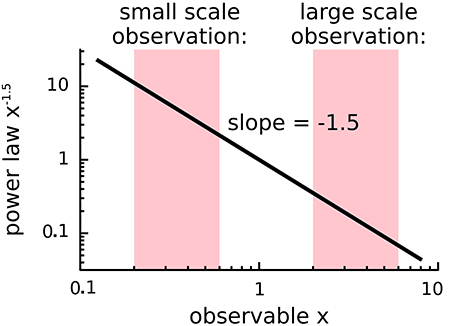
\includegraphics[width=\imsize]{fnsys-08-00166-g003.jpg}
	\caption[Representación gráfica de la independencia de escala de las leyes de potencia en una distribución de datos.]{Representación gráfica de la independencia de escala de las leyes de potencia en una distribución de datos, donde se ha utilizado la ley de potencia $f(x) = x^{-\alpha}$  con un exponente crítico de $\alpha=-1.5$ y una escala logarítmica en el eje $x$. La figura muestra que, independientemente del rango o escala utilizada para medir la distribución, se observa una ley de potencia con el mismo exponente crítico.} 	\label{fig:leypotencia}
\end{figure}


La hipótesis de criticidad en experimentos y simulaciones se basa en la presencia de leyes de potencia, que se espera se manifiesten en la mayoría de los sistemas críticos. Sin embargo, la existencia de leyes de potencia por sí sola no es suficiente para probar la criticidad \cite{goldstein_problems_2004,priesemann_can_2018}, ya que estas leyes también pueden ser explicadas por mecanismos no críticos \cite{touboul_can_2010,markovic_power_2014,noauthor_critical_2006,beggs_being_2012}. Por tanto, la identificación de leyes de potencia es un asunto delicado que requiere procedimientos de ajuste avanzados, debido a la dificultad para diferenciarlas de otras distribuciones de colas pesadas.\\

Las distribuciones de cola pesada son aquellas distribuciones de probabilidad cuyas colas son \textquote{más pesadas} que la distribución exponencial, siendo la gaussiana un subtipo de esta última. Entre los ejemplos de distribuciones de cola pesada se encuentran la distribución de Fisher-Tippett (doble exponencial), la distribución logarítmica normal y la distribución de Weibull, entre otras. Aunque se espera la presencia de leyes de potencia en sistemas críticos, estas distribuciones también pueden presentarse en otros sistemas no críticos. Por ende, para una mejor comprensión de la relevancia de las distribuciones de cola pesada en la neurociencia, se sugiere consultar la obra de Roberts et al  \cite{roberts_heavy_2015}.\\

Para abordar esta problemática, los investigadores han tenido acceso a metodologías estadísticas más sofisticadas gracias a los trabajos realizados por Clauset et al  \cite{clauset_power-law_2009} y otros estudios posteriores \cite{klaus_statistical_2011,markovic_power_2014}. Estas metodologías permiten distinguir las leyes de potencia de otras distribuciones de colas pesadas y evaluar su presencia en sistemas críticos. Sin embargo, es importante tener en cuenta que las leyes de potencia se truncan en sistemas de tamaño finito \cite{bonachela_self-organization_2010} y pueden verse afectadas por el submuestreo \cite{ribeiro_undersampled_2014}. Por lo tanto, es necesario emplear medidas cuantitativas para evaluar la diferencia entre las distribuciones de probabilidad acumulada experimental y ajustada por ejemplo  a través del parámetro $\kappa$ \cite{shew_neuronal_2009}.



\subsection{Escalamiento de  la ley de potencia de las avalanchas neuronales }

Beggs y Plenz demostraron experimentalmente que el comportamiento espontáneo de las redes corticales in vitro exhibe características consistentes con dinámicas críticas en su estudio histórico sobre avalanchas neuronales en cortes corticales interconectados con arreglos de microelectrodos (\gls{MEA}) \cite{beggs_neuronal_2003} . Una avalancha neuronal es una duración de actividad persistente que se propaga a través de la red y está marcada por períodos de silencio que preceden y siguen al período activo (ver \Cref{fig:avalancha}). En el caso de sistemas in vitro (es decir, cortes o cultivos disociados), la \textquote{actividad } puede referirse a los picos de mayor frecuencia o el \gls{LFP} de menor frecuencia, ya que se han estudiado ambas modalidades.\\

\begin{figure}[ht]
	\centering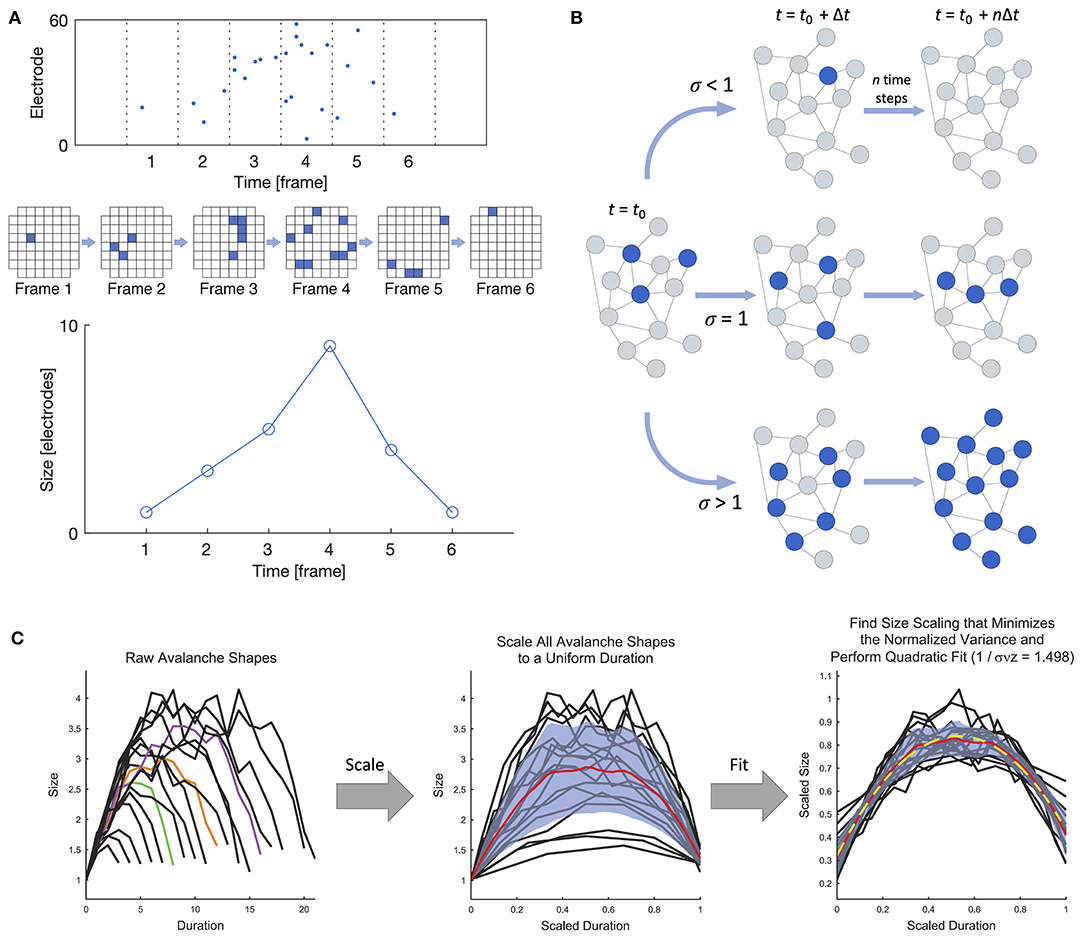
\includegraphics[width=\imsize]{fncom-15-611183-g002.jpg}
	\caption[Definición de avalancha neuronal y ejemplos de medidas empíricas de criticidad. ]{Definición de avalancha neuronal y ejemplos de medidas empíricas de criticidad. 
		(a) Se presenta la definición de avalancha neuronal, mostrando en el panel superior un gráfico rasterizado dividido en intervalos de tiempo. La avalancha representada abarca seis fotogramas activos, precedidos y seguidos por fotogramas inactivos. A continuación, se muestra una vista alternativa de la actividad en los seis marcos, en la que cada cuadrado representa un electrodo activo en una cuadrícula de 8x8. El panel inferior exhibe la definición de la forma de avalancha, la cual se obtiene a partir del número de electrodos activos en cada cuadro.
		(b) Se ilustra la relación de ramificación, en la cual los nodos azules representan actividad activa y los grises, inactiva. En una relación de ramificación de 1, la actividad persiste sin sobrecargar el sistema.
		(c) Se observa el colapso de forma en un sistema crítico, donde todas las avalanchas deberían mostrar el mismo perfil de forma temporal media en diferentes escalas de tamaño.
		Esta representación ha sido adaptada de Heiney et al.  \protect{\cite{heiney_criticality_2021}}.} 	\label{fig:avalancha}
\end{figure}


El escalamiento de la ley de potencia del tamaño $S$ y la duración $T$ de las avalanchas neuronales es un sello distintivo de la criticidad en las redes neuronales. Es decir, $P(S) \propto S^{-\alpha}$  y $P(T) \propto T^{-\beta}$, donde $P(·)$  es la función de distribución de probabilidad. El tamaño se define generalmente como el número de electrodos o neuronas activados, y la duración es el número de intervalos de tiempo activos. Los exponentes de la ley de potencia del tamaño y la duración son aproximadamente $\alpha=1.5$ y $\beta= 2.0$, respectivamente, cuando se selecciona el ancho del intervalo de tiempo para que se corresponda con el intervalo promedio entre picos. Sin embargo, la escala de la ley de potencia debe persistir en un rango de resoluciones temporales cercano al orden de magnitud del intervalo promedio entre picos, con el exponente $\alpha$ cambiando sistemáticamente con el tamaño del intervalo de tiempo seleccionado \cite{beggs_neuronal_2003,pasquale_self-organization_2008}. La escala de ley de potencia también debe mantenerse cuando se considera una resolución espacial de grano más grueso, utilizando solo un subconjunto de todos los puntos de registro. Las redes neuronales pueden mostrar varios puntos críticos dinámicos únicos, de los cuales solo uno es la transición de fase que da lugar a las avalanchas neuronales. Por lo tanto, es crucial considerar el contexto más amplio y no limitarse a la transición de fase en sí misma \cite{kanders_avalanche_2017}.







\subsection{Parámetro de ramificación}



En la teoría de los procesos de ramificación \cite{harris_theory_1963} se utiliza una medida común, la relación de ramificación $\sigma$, para evaluar el número de descendientes y ancestros en un sistema. En particular, esta medida establece la proporción entre el número de descendientes y el número de ancestros, en el que la actividad en un electrodo o neurona ancestro precede inmediatamente a la actividad en un electrodo o neurona descendiente \cite{beggs_neuronal_2003}. En un sistema en estado crítico, la relación de ramificación se aproxima a $1$, lo que permite que la actividad fluya a través de la red sin extinguirse ($\sigma < 1$) o saturar toda la red ($\sigma > 1$), tal como se muestra en la \cref{fig:avalancha}. Por tanto, la presencia de una relación de ramificación $\sigma = 1$ en respuesta a una excitación artificial en un sistema lo suficientemente inactivo puede considerarse como una evidencia de criticidad.\\

No obstante, es importante destacar que, en comparación con otras características, la evidencia proporcionada por una relación de ramificación de uno es relativamente débil. Esto se debe a que dicha relación no implica necesariamente una dinámica crítica, ya que también puede ser observada en estados supercríticos \cite{hesse_self-organized_2014}. Por lo tanto, se requiere de un análisis más riguroso que permita distinguir entre ambos estados.


\subsection{Colapso de forma}


La dinámica de los sistemas críticos se caracteriza por la presencia de avalanchas de actividad, que exhiben una naturaleza autosimilar o fractal. Se espera que la \textquote{forma} de la actividad de la avalancha se comporte como un fractal en dichos sistemas. En un estado crítico, se espera que todas las avalanchas muestren el mismo perfil temporal medio en todas las escalas. El perfil temporal de una avalancha se define como el número de sitios activos en función del tiempo. Para un sistema en estado crítico, los perfiles temporales de todas las avalanchas colapsan en la misma forma de perfil cuando se escala espacio-temporalmente con un exponente de escala$\gamma$ cercano a $2$(\Cref{fig:avalancha}). Esta propiedad se describe por  $ \left\langle S\right\rangle(T) \propto T^{-\gamma}$, donde $\left\langle S\right\rangle(T)$  representa el tamaño promedio de todas las avalanchas de una duración determinada $T$.\\

Se puede encontrar información detallada sobre el colapso de la forma en la literatura científica, como en Sethna et al \cite{sethna_crackling_2001} y Friedman et al \cite{friedman_universal_2012}. Además, Miller et al \cite{miller_scale-invariant_2019} proporciona una demostración experimental del colapso de la forma en primates no humanos. El coeficiente de criticidad (DCC) de Ma et al \cite{ma_cortical_2019} se relaciona con el concepto de colapso de forma y se calcula a partir de la diferencia entre el exponente de escala $\gamma$, obtenido a partir de datos empíricos mediante regresión lineal, y el valor esperado obtenido a partir del exponente de ley de potencia $\alpha$ de la distribución de tamaños.


\subsection{Submuestreo espacial}

Debido a la naturaleza intrínseca de la observación de los sistemas neuronales, se ve limitada la capacidad de muestrear todos los componentes del sistema. Como consecuencia, se puede obtener únicamente una muestra espacialmente submuestreada del sistema, la cual puede resultar insuficiente para obtener conclusiones precisas acerca de la dinámica subyacente del sistema. Para abordar este problema, se han desarrollado métodos que involucran el escalado del submuestreo espacial \cite{levina_subsampling_2017} y el uso de un estimador invariante de submuestreo \cite{wilting_inferring_2018}. Estos métodos permiten la evaluación precisa de los estados dinámicos de sistemas submuestreados, incluso en situaciones donde el número de componentes muestreados es significativamente menor que el número total de componentes del sistema.



\subsection{Correlación temporal de largo alcance, ralentización crítica y flickering}


En sistemas críticos, la respuesta del sistema a los estímulos externos se maximiza, lo que se conoce como rango dinámico o correlación dinámica. La criticidad del sistema genera retornos geométricos al estado estacionario \cite{hesse_self-organized_2014}, lo que resulta en una correlación temporal de largo alcance \gls{LRTC} o memoria larga. La \gls{LRTC} puede medirse de diversas maneras, siendo los métodos más populares el exponente de Hurst, a través de varios estimadores, y   \gls{DFA}  \cite{hardstone_detrended_2012}. Este último produce un exponente de escala durante un período de tiempo determinado. Un exponente de escala entre $0.5$ y $1$, con un buen ajuste, indica que la serie de tiempo exhibe \gls{LRTC} durante ese período.\\

La tasa geométrica de retorno al estado estacionario también se conoce como desaceleración crítica \cite{scheffer_early-warning_2009}. En el punto crítico, la correlación dinámica del sistema diverge de tal manera que se producen avalanchas, es decir, actividad de la red, en todas las escalas del sistema \cite{hesse_self-organized_2014}. Este fenómeno se debe a que la fluctuación en la criticidad del sistema se propaga a través de la red, generando actividad a diferentes escalas. Además, en la transición crítica, surge el fenómeno del flickering, que se produce cuando el ruido permite que un sistema migre de un lado a otro entre dos cuencas atractoras \cite{wang_flickering_2012}. En este caso, el sistema se encuentra en un estado metaestable y su comportamiento no puede ser descrito por un solo atractor.




\subsection{Ruido $(1/ f )$ y ley de potencia}

Los sistemas críticos exhiben respuestas geométricas superpuestas a entradas débiles, lo que produce ruido $1/f$, también conocido como ruido rosa, ruido de ley de potencia o ruido flicker. La dependencia de largo alcance o memoria larga se utiliza a menudo como sinónimo de estos términos, ya que se trata de fenómenos idénticos. El término ruido $1/f$ se refiere al espectro de potencia $S(f)$ de una serie temporal, el cual sigue una ley de potencia de la forma $S( f ) = \alpha f^{-\beta}$. Históricamente, se han identificado los casos $\beta=0$, $\beta=1$, $\beta=2$ como ruido \textquote{blanco}, ruido \textquote{rosa}  y ruido \textquote{marrón}, respectivamente \cite{li_fractal_2005}. El ruido $1/f$ se acepta comúnmente en el rango  $0.5 < \beta < 1.5$. Si bien todos los sistemas críticos deben exhibir ruido $1/f$, no todo el ruido $1/f$ es indicativo de criticidad \cite{bedard_does_2006,hesse_self-organized_2014}. 



\section{Discusión}

La hipótesis de la criticidad neuronal está motivada por la relación entre la criticidad y las propiedades computacionales óptimas. La hipótesis está respaldada por experimentos que observaron características de criticidad para una amplia gama de animales, en varios estados de conciencia y en muchas escalas experimentales diferentes, desde grabaciones de unas pocas neuronas hasta todo el cerebro.  Sin embargo, se ha señalado que algunas pruebas pueden ser engañosas \cite{clauset_power-law_2009} y podrían explicarse potencialmente por mecanismos alternativos \cite{botcharova_power-law_2012,galinsky_neuronal_2023}. Algunos estudios experimentales también informan resultados negativos donde no se observaron características de criticidad en la actividad neuronal  \cite{yu_scale-invariant_2014,bedard_does_2006,dehghani_avalanche_2012}. En general, la relación entre el marco teórico y su realización biológica sigue sin estar clara.  Con base con lo presentando en este capitulo , consideramos que la criticidad es preferible a las explicaciones alternativas porque proporciona una explicación motivada por la evolución para varias observaciones que de otro modo estarían desconectadas.\\

A pesar de las advertencias antes mencionadas, la creciente investigación empírica y de modelado respalda claramente la opinión de que la dinámica neuronal probablemente ocurra cerca de inestabilidades críticas. El reconocimiento de las limitaciones de este nuevo campo simplemente muestra que ha madurado más allá de las primeras etapas. El objetivo principal de este capitulo fue el de realizar una revisión de la relevancia, limitaciones y aplicaciones de la hipótesis de criticidad neuronal.   En la mayor parte de estas investigaciones tanto en los experimento  como en  el modelado  la criticidad fue analizada a nivel \textquote{macroscópico} es decir en grandes regiones del cerebro particularmente en la corteza cerebral.  Desafortunadamente no existen experimentos que analicen la criticidad neuronal a nivel de todo el sistema nervioso de un organismo. Esto en parte es debido a que las técnicas que realizan  un seguimiento de la actividad neuronal de todo el sistema nervioso  son  recientes y están limitadas a organismos simples como por ejemplo el C. elegans \cite{kato_global_2015,kaplan_nested_2020,yemini_neuropal_2021}. Otro inconveniente es que aun teniendo toda la dinámica neuronal global  de un organismo esta debe modificarse  mediante fármacos, manipulación genética u otras técnicas para verificar que el estado optimo es el cercano al estado critico, por lo que muchos animales deben utilizarse y adaptar varios protocolos experimentales a estos cambios. Por otro lado los modelos que analizan la dinámica  critica  con el  conectoma completo del C. elegans son escasos  \cite{ciftci_synaptic_2018} y ninguno de ellos  analiza la dinámica critica de todo el sistema nervioso en ausencia de estímulos y los contrasta con resultados experimentales.\\

Sabiendo las limitaciones experimentales y los pocos modelos que analizan la dinámica critica a nivel global esta parte de la tesis busca  aportar  a estas limitaciones proponiendo una solución a la pregunta ¿Existe una dinámica critica a nivel global en el C. elgans  en ausencia de estímulos
externos?. Para responder a esta pregunta  en primer lugar  se aplicaran  algunas de las métricas experimentales de criticidad presentadas en este capitulo  en  datos experimentales de la dinámica neuronal global de  gusanos inmovilizados suministrados por (Kato et al) \cite{kato_global_2015}, (Kaplan et al)  \cite{kaplan_nested_2020} y neuropal \cite{yemini_neuropal_2021}.  El  objetivo especifico es analizar en que región se encuentra los datos experimentales de las   dinámicas neuronales del C. elgans.  Nuestra hipótesis de trabajo es que aun en un organismo tan pequeño como lo es el C. elegans la dinámica neuronal se encuentran en un régimen dinámico cercano al punto crítico de una transición de fase de segundo orden.\\


Por otro lado para superar las limitaciones experimentales de no poder manipular en tiempo real la dinámica neuronal y  tener un mayor control de los parámetros del sistema se plantea un modelo utilizando  el Conectoma  realizado por Cook y coautores  \cite{cook_whole-animal_2019} el cual abarca  todas las conexiones  neuronales  del C. elegans  junto a una  dinámica neuronal descrita por una regla dinámica no lineal muy simple la cual es una  adaptación del modelo neural Greenberg-Hastings introducida por Haimovici y coautores  \cite{haimovici_brain_2013}.   El  objetivo específico busca cuantificar la dinámica critica  en términos de un parámetro de orden   que emerge al manipular tanto los parámetros de  la dinámica neuronal  como el parámetro de control del sistema.  La hipótesis de trabajo es que los patrones espacio temporales observados de manera experimental en la actividad cerebral en ausencia de estímulos  solo pueden ser descriptos por un modelo de red neural si la misma se encuentra en un estado crítico. Finalmente, como objetivo específico buscaremos establecer relaciones entre los resultados experimentales y  nuestro modelo. En el siguiente capitulo se introducirá  mediante la teoría de percolaciones  el parámetro de orden que  nos permitirá caracterizar la transición de fase que surge al aplicar una dinámica critica al conectoma del C. elegans. 









%%% Local Variables: 
%%% mode: latex
%%% TeX-master: "template"
%%% End: 


\appendix
\chapter{Diferenciación numérica de datos ruidosos y no suaves}\label{C:ap1}
\chapterquote{Distinguishing the signal from the noise requires both scientific knowledge and self-knowledge: the serenity to accept the things we cannot predict, the courage to predict the things we can, and the wisdom to know the difference.}{Nate silver, 2012}
\graphicspath{{figs/apendice_derivada_ruidosa}}
%%%%%%%%%%%%%%%%%%%%%%%%%%%%%%%%%%%%%%%%%%%%%%%%%%%%%%%%%%%%%%%%%%%%%%%%




El cálculo de derivadas de datos de mediciones ruidosas es omnipresente en las ciencias físicas, de ingeniería y biológicas, y suele ser un paso fundamental en el desarrollo de modelos dinámicos o el diseño del control. Por desgracia, la formulación matemática de la diferenciación numérica suele estar mal planteada, y los investigadores recurren a menudo a un proceso ad hoc para elegir uno de los muchos métodos computacionales y sus parámetros \cite{9241009}. Existe un amplio y variado conjunto de herramientas matemáticas para estimar las derivadas de datos ruidosos, la mayoría de las cuales se formulan como un problema mal planteado regularizado por algunas restricciones de suavizado apropiadas.  En este apéndice se considera el problema de diferenciar una función especificada por datos ruidosos. El método  elegido es la \gls{regularizacion} del proceso de diferenciación el cual evita la amplificación de ruido de los métodos de diferencias finitas.  La regularización de variación total se utiliza por que permite soluciones discontinuas. El algoritmo simple resultante diferencia con precisión las funciones ruidosas, incluidas aquellas que tienen una derivada discontinua.

\section{Introducción}

En muchas aplicaciones científicas, es necesario calcular la derivada de funciones especificadas por datos. Las aproximaciones por diferencias finitas convencionales amplificarán en gran medida cualquier ruido presente en los datos. La eliminación del ruido de los datos antes o después de la diferenciación no suele dar resultados satisfactorios \cite{chartrand_numerical_2011}.  

Un método que da buenos resultados es regularizar el propio proceso de diferenciación. Esto garantiza que la derivada calculada tendrá cierto grado de regularidad, hasta un punto que a menudo se puede controlar ajustando los parámetros. Un marco común para ello es la regularización de Tikhonov \cite{1570291226450870144} del problema inverso correspondiente. Es decir, la derivada de una función  $f$ en  $[0,L]$ es el minimizador del funcional

\begin{equation}\label{eq:81}
F(u)=\alpha R(u) +DF\left(Au-f\right)
\end{equation}


donde  $R(u)$  es un término de regularización o penalización que penaliza la irregularidad en  $u$ , $Au(x)=\int_{0}^{x}u$  es el operador de antidiferenciación,  $DF\left(Au-f\right)$  es un término de fidelidad de los datos que penaliza la discrepancia entre $Au$ y $f$, y $\alpha$  es un parámetro de regularización que controla el equilibrio entre los dos términos.  El término de fidelidad de los datos $DF$ suele ser el cuadrado de la norma $L^2$, $DF=\int_{0}^{L} \left| \cdot \right|^2$ , como corresponde si $f$  tiene ruido gaussiano blanco aditivo. Se pueden utilizar otros términos de fidelidad de datos si el ruido tiene una distribución diferente y conocida.

\section{ Regularización de variación total }

La regularización de variación total se debe a Rudin et al. en \cite{rudin_nonlinear_1992}. Desde entonces ha encontrado muchas aplicaciones en el tratamiento de imágenes.  Chartrand \cite{chartrand_numerical_2011}  propuso  utilizar la regularización de variación total en la \cref{eq:81}. Así, se puede calcular  la derivada de  $f$  en  $[0,L]$  como el minimizador del funcional 

\begin{equation}\label{eq:82}
	F(u)=\alpha\int_{0}^{L}\left|u^\prime \right| +\frac{1}{2}\int_{0}^{L}\left| Au-f\right|^2. 
\end{equation}

Suponemos que $f\in L^2$ (una suposición vacía en el caso discreto), y por conveniencia que $f(0)=0$ (en la práctica simplemente restamos $f(0)$ de $f$ ). La función $F$ está definida en $BV[0,L]$, el espacio de funciones de variación acotada.   El uso de la variación total consigue dos cosas. Suprime el ruido, ya que una función ruidosa tendrá una variación total grande. Tampoco suprime las discontinuidades de salto, a diferencia de las regularizaciones típicas. Esto permite el cálculo de derivadas discontinuas y la detección de esquinas y bordes en datos ruidosos.

\section{Implementación numérica}

Un enfoque sencillo para minimizar \cref{eq:82} es el descenso del gradiente. Esto equivale a evolucionar a estacionariedad la EDP obtenida a partir de la ecuación de Euler-Lagrange:

\begin{equation}\label{eq:83}
u_t=\alpha\frac{d}{dx}\frac{u^\prime}{\left| u^\prime\right| }-A^T\left(Au-f\right),
\end{equation}

donde $A^Tv(x)=\int_{x}^{L}v$ es el $L^2$-adjunto de $A$. Sustituyendo $\left|u^\prime \right|$  en el denominador por $\sqrt{\left(u^\prime\right)^2+\epsilon}$ para algún valor pequeño de $\epsilon>0$  evita la división por cero. Típicamente, La \cref{eq:83} se implementa con marcha temporal explícita, con $u_t$  discretizada como $\left(u_{n+1}-u_n\right)/\Delta t$ para algún valor fijo de $\Delta t$. El problema con la \cref{eq:83}  es que la convergencia es lenta. Un algoritmo más rápido es el método de difusividad retardada de Vogel y Oman \cite{vogel_iterative_1996}. La idea es sustituir en cada iteración de  la \cref{eq:83}  el operador diferencial no lineal $u\mapsto(d/dx)\left(u^\prime/ \left|u^\prime \right|\right)$ por el operador lineal $u\mapsto(d/dx)\left(u^\prime/\left|u^\prime_n \right| \right)$ . Se ha demostrado que el algoritmo converge al minimizador de $F$.


Menos sencilla es la elección del parámetro de regularización $\alpha$. Un enfoque consiste en utilizar el principio de discrepancia: la diferencia cuadrática media entre $Au^*$ y $f$  debe ser igual a la varianza del ruido en  $f$ . Esto tiene el efecto de elegir la solución más regular del problema inverso mal planteado $Au=f$  que sea consistente con los datos  $f$ . En la práctica, el ruido en $f$  no suele conocerse, pero la varianza del ruido puede estimarse comparando $f$ con una versión suavizada de  $f$. El otro enfoque consiste simplemente en utilizar el método de ensayo y error, ajustando  $\alpha$  para obtener el equilibrio deseado entre la supresión de las oscilaciones y la fidelidad a los datos. En la siguiente sección, veremos un ejemplo que muestra el efecto del valor de $\alpha$.


\section{Ejemplo}

Para el calculo de la derivada numérica regularizada por variación total (TVDiff) se utilizo la implementación en Python realizada por Simone Sturniolo \footnote{La documentación esta disponible en \url{https://github.com/stur86/tvregdiff}}. Para ver el funcionamiento del algoritmo utilizamos  un ejemplo sencillo.  Sea $f_0(x)=\left| x-1/2\right|$ , definida en 100 puntos uniformemente espaciados en  $[0,1]$ . Obtenemos  $f$  añadiendo ruido gaussiano de desviación estándar $0.05$. La \cref{f:funcion_ruidosa} muestra el  $f$ . En primer lugar, mostramos en la \cref{f:derivada_centrada} el resultado de calcular  $u(x)=df/dx$ por diferencias finitas. Comparamos los resultados con la derivada verdadera  $u(x)=sgn(x)$ y una aplicación ingenua de diferencias finitas $u_{FDM}$. Incluso  con un ruido de amplitud moderada como el de este ejemplo, una aplicación ingenua como lo es $u_{FDM}$ produce estimaciones de la derivada que son demasiado ruidosas para ser útiles.


\begin{figure}[h!]
\centering{}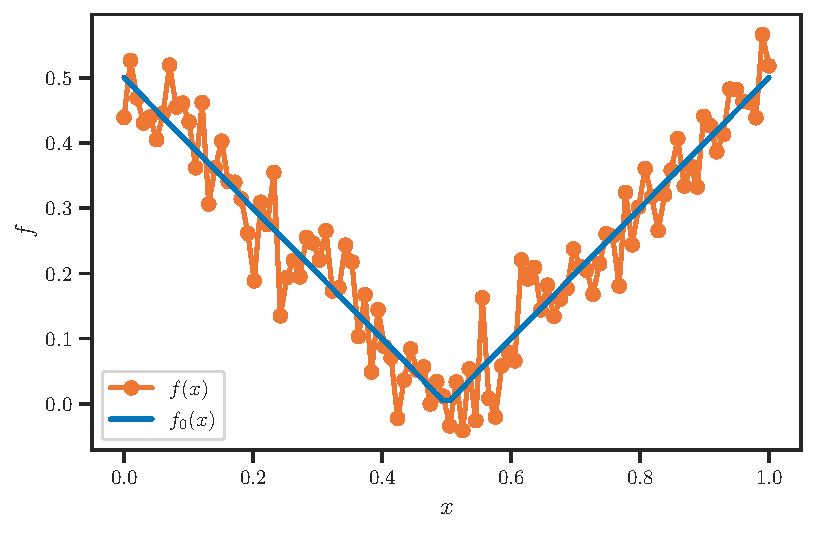
\includegraphics[width=\imsize]{funcion_ruidosa.pdf}
\caption{La función $f$ obtenida a partir de  $f_0=\left| x-1/2\right|$   añadiendo ruido gaussiano de desviación estándar $0.05$}\label{f:funcion_ruidosa}  
\end{figure}

\begin{figure}[h!]
	\centering{}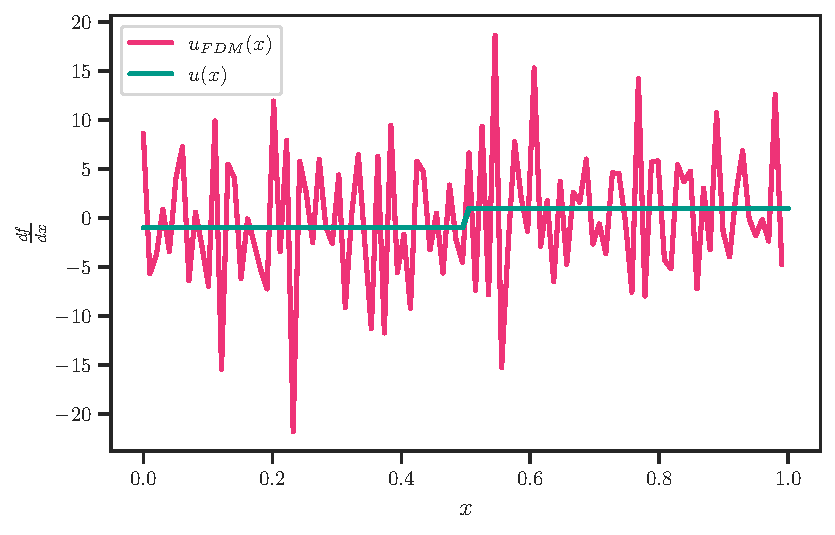
\includegraphics[width=\imsize]{derivada_centrada.pdf}
	\caption{El cálculo de $u_{FDM}(x)$ con diferencias finitas amplifica enormemente el ruido.}\label{f:derivada_centrada}  
\end{figure}


Ahora, se implementa la TVDiff, dada por la \cref{eq:82}. Para ver como varían los resultados con el parámetro de regularización $\alpha$, se comparan 3 valores de este. En todos los casos se utilizan los parámetros $\epsilon=$\num{1e-6} y 7000 iteraciones.  Con un   $\alpha=$\num{1e-4}  tan bajo (Figura (a)) el ruido residual en el proceso de diferenciación aún se amplifica lo suficiente como para dar un resultado insatisfactorio. Con una regularización más fuerte $\alpha=2$ el resultado es mucho mas suave y similar al resultado teórico.  A pesar de la fuerte suavización, se captan bien las rápidas subidas y bajadas del derivado. Éste es el efecto de la regularización, cuya elección sirve para determinar la magnitud de la fluctuación que se considera insignificante. Aunque el suavizado mitiga los errores, también puede introducir sesgos.  Finalmente un parámetro mas optimizo seria $\alpha=0.2$, la forma general de $f^\prime_0$ se captura casi perfectamente. El salto está correctamente localizado. La única imprecisión es el tamaño del salto: hay una pérdida de contraste, típica de la regularización de totalización en presencia de ruido. Disminuir el tamaño del salto reduce el término de penalización en la \cref{eq:82}, a expensas de aumentar el término de fidelidad de los datos.


\begin{figure}[h!]
	\centering{}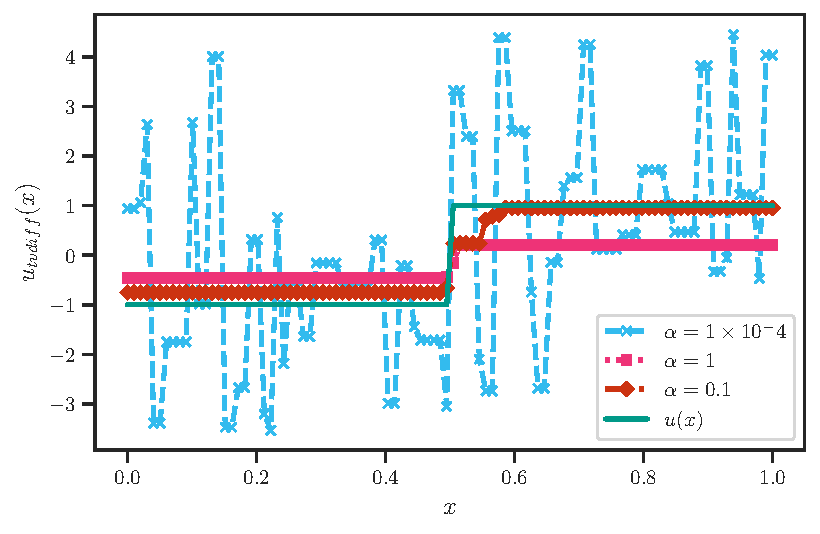
\includegraphics[width=\imsize]{derivada_regularizadas.pdf}
	\caption[Resultados de la derivada con diversos valores del parámetro de regularización. ]{Resultados de la derivada con diversos valores del parámetro de regularización. Los resultados se comparan con el valor teórico $u(x)$ que en este grafico es la linea color verde. Con un parámetro de regularización bajo $\alpha=0.1$ (linea color celeste) el resultado es ruidoso e impreciso.  Por otra parte un parámetro alto $\alpha=1$ de regularización puede introducir sesgos (linea color rosa). Una regularización optima  con $\alpha=0.1$  produce una derivada sin ruido con un salto agudo correctamente localizado. La discrepancia de los valores de  $\pm 1$  se deben a la pérdida de contraste, un artefacto de los métodos de variación total en presencia de ruido.}\label{f:derivada_regularizada}  
\end{figure}


También se muestra el resultado de aplicar el operador de antidiferenciación al valor de las derivadas calculadas (\cref{f:integral_derivada_regularizada}) y lo comparamos con el de la teórica. Como sucede en la derivada el mejor resultado es cuando $\alpha=0.1$. 


\begin{figure}[h!]
	\centering{}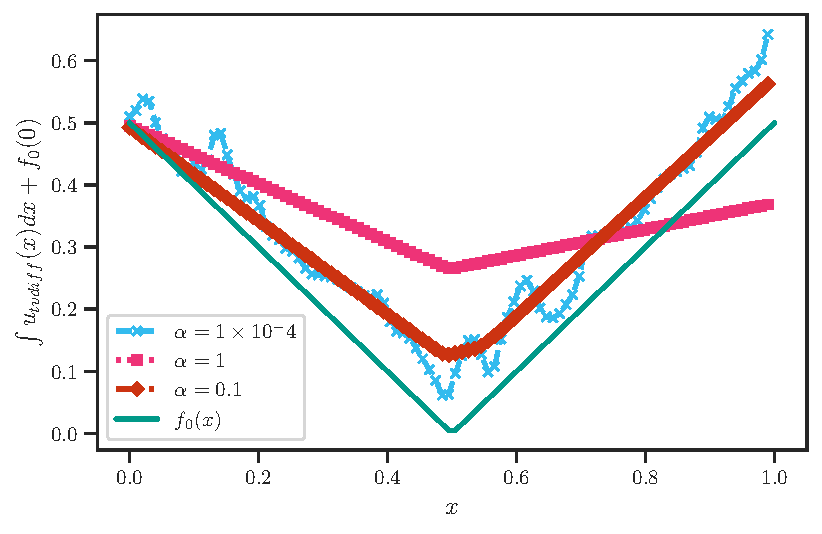
\includegraphics[width=\imsize]{integral_derivada_regularizadas.pdf}
	\caption[Resultados de la anti-derivada aplicada la derivada regularizada con diversos valores del parámetro de regularización. ]{Resultados de la anti-derivada aplicada la derivada regularizada  con diversos valores del parámetro de regularización. Los resultados se comparan con el valor real $f_0(x)$ que en este grafico es la linea color verde. Con un parámetro de regularización bajo $\alpha=0.1$ (linea color celeste) se obtiene una función ruidosa tal como $f(x)$.  Por otra parte un parámetro alto $\alpha=1$ de regularización puede introducir sesgos (linea color rosa) el cual desviá el resultado de la función real. Una regularización mas optima  como $\alpha=0.1$  produce un resultado  muy similar a la función exacta $f_0$}\label{f:integral_derivada_regularizada}  
\end{figure}

\section{Elección de parámetros óptimos}\label{sec:parametors_optimos}

Como se explico en la anterior sección para obtener un resultado optimo se debe realizar una elección adecuada de los parámetros. Se debe buscar que el valor de este parámetro no sea muy alto  lo cual suavizaría la derivada  en exceso dando como resultado  perdidas de información que pueden ser relevantes.  Por otra parte  un parámetro demasiado bajo al igual que las diferencias finitas da un resultado  ruidoso. Sin embargo, el nivel y el tipo de regularización suelen imponerse de forma ad hoc, por lo que actualmente no existe un \textquote{mejor método} consensuado para obtener las derivadas \textquote{mejor ajustadas}. Para solventar este problema  Van Breugel et al \cite{van_breugel_numerical_2020} adoptaron un enfoque basado en principios y propusieron  un marco de optimización multiobjetivo para elegir los parámetros que minimizan una función de pérdida para equilibrar la fidelidad y la suavidad de la estimación de la derivada. Este  marco presenta tres ventajas significativas. En primer lugar, la tarea de seleccionar múltiples parámetros se reduce a la elección de un único hiperparámetro. En segundo lugar, cuando se desconocen los datos reales, se proporciona una heurística para seleccionar este hiperparámetro basándonos en el espectro de potencia y la resolución temporal de los datos. En tercer lugar, el valor óptimo del hiperparámetro es coherente con los distintos métodos de diferenciación, por lo que este enfoque unifica métodos de diferenciación numérica muy diferentes y facilita la comparación imparcial de sus resultados. Por último, se proporciona una amplia biblioteca Python de código abierto, pynumdiff \footnote{La documentación se puede encontrar en  el siguiente link \url{https://github.com/florisvb/PyNumDiff}}, para facilitar su aplicación a diversos conjuntos de datos. El  objetivo de este paquete es desarrollar un enfoque general para elegir metódicamente parámetros que equilibren la necesidad de minimizar tanto el error como el sesgo. 

Para lograr este objetivo se minimiza una función de pérdida consistente en una suma ponderada de dos métricas calculadas a partir de la estimación de la derivada $\hat{\dot{x}}$: la fidelidad de la integral de la derivada y su suavidad. El procedimiento es el siguiente:  dadas unas mediciones ruidosas $y$, buscamos estimar la derivada en el tiempo del sistema dinámico que subyace a las mediciones $\hat{\dot{x}}$ . Cuando la verdadera $\dot{x}$ es desconocida, proponemos elegir el conjunto de parámetros $\Phi$ (para cualquier algoritmo numérico dado)   que minimicen la siguiente función de pérdida, 

\begin{equation}\label{eq:ap:1}
	L = \text {RMSE} \bigg (\text {trapz}({\hat {\dot {\mathbf {x}}}} (\Phi)) + \mu, {\mathbf {y}} \bigg) + \gamma \bigg ({TV}\big ({\hat {\dot {\mathbf {x}}}} (\Phi)\big)\bigg),\qquad 
\end{equation}


donde  RMSE es el error cuadrático medio,

\begin{equation}
\text {RMSE}({\hat {\dot {\mathbf {x}}}}, {\dot {\mathbf {x}}}) = \lVert ({\hat {\dot {\mathbf {x}}}} - {\dot {\mathbf {x}}})\rVert _{2},
\end{equation}

$\lVert{\cdot}\rVert _{2}$ es la 2-norma  del vector.  $\text{trapz}(\cdot)$ es la integral numérica trapezoidal en tiempo discreto, $\mu$ resuelve la constante de integración desconocida, 

\begin{equation} 
	\mu =\frac {1}{m}\sum _{k=0}^{m}\bigg (\text {trapz}({\hat {\dot {\mathbf {x}}}} (\Phi)) - {\mathbf {y}} \bigg),
	\end{equation}
	
$\gamma$ es un hiperparámetro y   $TV$ es la variación total,

\begin{equation} \label{eq:ap:2}
	TV({\hat {\dot {\mathbf {x}}}}) = \frac {1}{m}\left \lVert{ {\hat {\dot {\mathbf {x}}}} _{0:m-1}- {\hat {\dot {\mathbf {x}}}} _{1:m}}\right \rVert _{1},
	\end{equation}
	
 $\left\lVert{\cdot}\right\rVert _{1}$  denota la norma $\ell_1$ y $m$ es el número de instantáneas temporales de los datos.  El primer término de la función de pérdida en la\Cref{eq:ap:1} promueve la fidelidad de la estimación de la derivada asegurando que la integral de la estimación de la derivada se mantiene similar a los datos, mientras que el segundo término promueve la suavidad de la estimación de la derivada. Si $\gamma$ es cero, la función de pérdida simplemente devuelve la derivada por diferencias finitas. Los valores altos de $\gamma$ darán como resultado una estimación de la derivada más suave.  Esta función de pérdida reduce efectivamente el conjunto de parámetros $\Phi$ (que oscila entre 1 y 3 o más, dependiendo del método) a un único hiperparámetro $\gamma$. Desafortunadamente, $L$ no es convexo, pero se pueden utilizar rutinas de optimización manejables para resolver el conjunto de $\phi$ que minimizan $L$. Aquí se utiliza el método de Nelder-Mead \cite{nelder_simplex_1965}, un método de búsqueda directa simplex descendente que funciona bien para problemas de optimización no lineal. Para evitar que la optimización converja en mínimos incorrectos, lo utilizamos con múltiples condiciones iniciales. Finalmente este enfoque sugiere estas métricas como aproximaciones para minimizar el error y el sesgo de la derivada estimada, y en el articulo \cite{van_breugel_numerical_2020}  se demuestra que el barrido a través de los valores de un único hiperparámetro $\gamma$ produce estimaciones de la derivada que generalmente trazan el frente de Pareto de soluciones que minimizan el error y el sesgo.  Es importante destacar que este marco de optimización no asume ningún conocimiento de la verdadera derivada subyacente y reduce la tarea de seleccionar muchos parámetros de cualquier algoritmo de diferenciación a la resolución de una función de pérdida con un único hiperparámetro. 





%%% Local Variables: 
%%% mode: latex
%%% TeX-master: "template"
%%% End: 


\begin{biblio}
\bibliography{mibib}
\end{biblio}


\begin{postliminary}

\begin{seccion}{Publicaciones asociadas}
  \begin{enumerate}
  \item    Valencia Urbina, C. E., Cannas, S. A., \& Gleiser, P. M. (2023). Emergent dynamics in a robotic model based on the Caenorhabditis elegans connectome. Frontiers in neurorobotics, 16, 1041410. https://doi.org/10.3389/fnbot.2022.1041410
  
  \end{enumerate}
\end{seccion}

\begin{seccion}{Agradecimientos}
A todos los que se lo merecen, por merecerlo
\end{seccion}

\end{postliminary}

\end{document}

